\subsection{graphisme}
\par Cr�er un jeu, ce n'est pas seulement le d�velopper, c'est aussi travailler son rendu graphique. Cette t�che, surement la plus compliqu�e, a �t� une rude �preuve. 
\par Le premier travail fut de trouver un fond au jeu, puis des sprites. Par la suite, nous devions cr�er de nombreux missiles. Il a donc fallu faire un travail titanesque sur photoshop dans le but d'apprendre, et de cr�er ces missiles.
\par Voici un exemple de rendu en jeu des sprites et des missiles:
\includegraphics{images/graphisme.jpg}
\par De nombreux missiles devaient �tre dessin�s, comme vous pouvez le voir ci dessous:
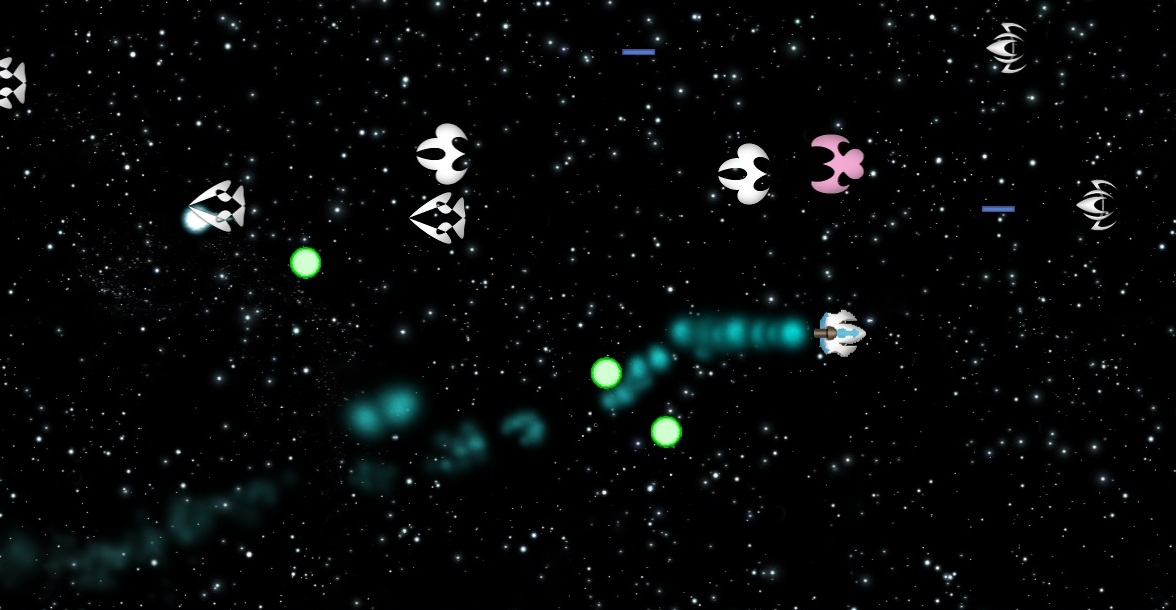
\includegraphics{images/graphisme3.jpg}
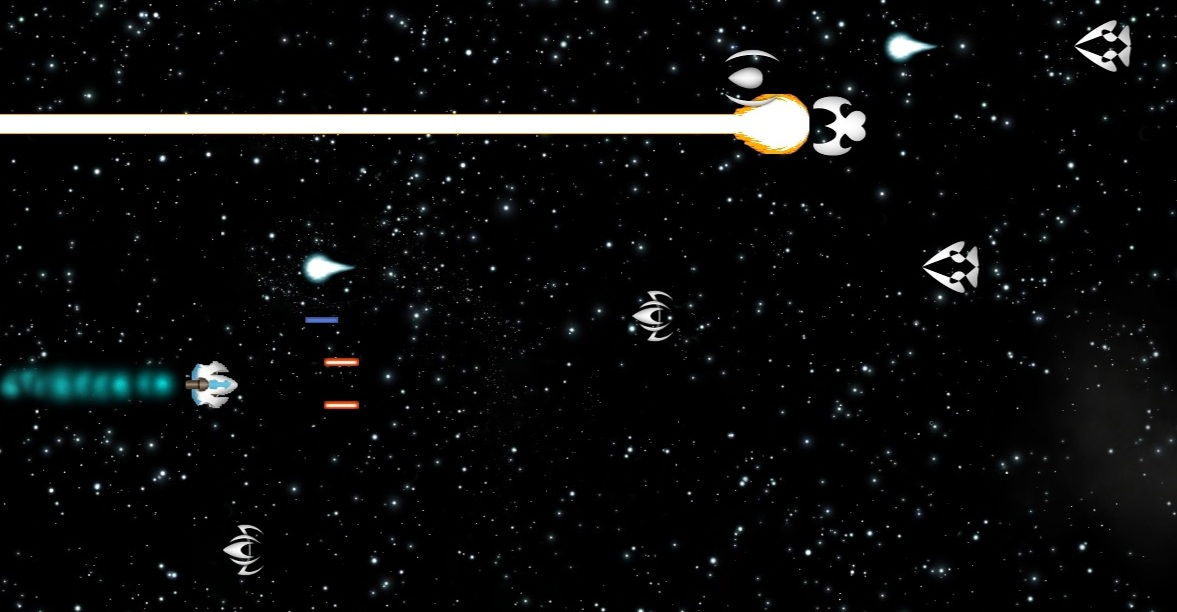
\includegraphics{images/graphisme2.jpg}
\par Le menu et le logo ont demand� aussi beaucoup de travail, pour un resultat final de bonne qualit�, que vous trouverez dans la partie Menu & Score.
\subsubsection{Interface}
\par L'interface quant � elle, devait �tre intuitive et agr�able � l'oeil. C'�tait LE d�fi graphique. 
\par Au d�part absente, elle est apparue d�s la soutenance 2 sous une forme plus compl�te:
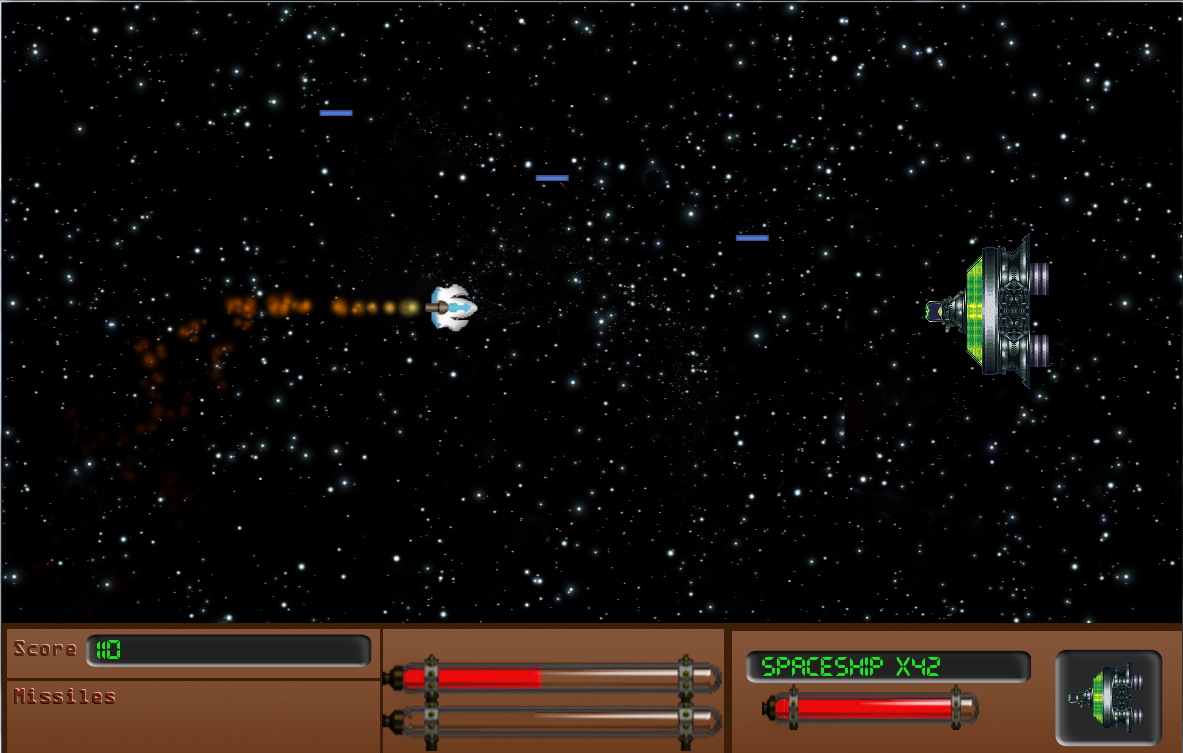
\includegraphics{images/hud1.png}
\par Vous pouvez y voir la vie du joueur, son score, et des informations sur le boss actuel. Toutefois, le plus dur rester � faire: Cr�er une interface intuitive. C'est pourquoi impl�menter les missiles dans l'interface ne fut pas une t�che simple, et nous devions rendre cela beau graphiquement pour ne pas heurter l'oeil du joueur.
\par Nous avons donc aussi d�cid� de rajouter une barre d'�nergie d�s la soutenance 3, permettant de tirer diff�rents missiles disponibles dans l'arsenal du joueur. Au final, l'interface est simple, intuitive, et jolie graphiquement:
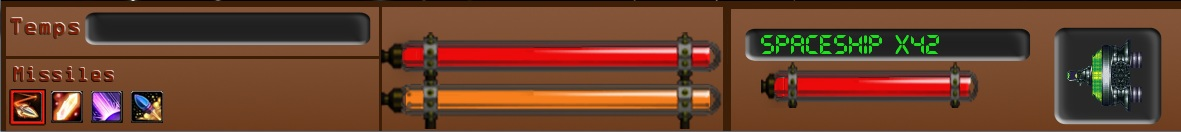
\includegraphics{images/interface.jpg}